\chapter{Contribuição: StarVZ sobre Spark} \label{ch:contribution}

A fase de pré-processamento do arcabouço StarVZ é similar a um fluxo de Ciência 
de dados. Nele, são carregadas e manipuladas várias tabelas, utilizando 
bibliotecas do pacote \texttt{tidyverse}. Este Capítulo fala sobre as diferenças 
propostas e realizadas no StarVZ, com o objetivo de otimizar o tempo de 
execução desta fase. Resumidamente, no lugar de tabelas R, utilizaremos tabelas
Spark (\emph{Spark Dataframes}) para o carregamento e manipulação de dados.
Na Seção \ref{sect:arch} são apresentadas as mudanças 
arquiteturais propostas e na Seção \ref{sect:implement}, detalha-se a 
implementação dessas mudanças.

\section{Arquitetura Proposta} \label{sect:arch}

A arquitetura da aplicação que este trabalho se propõe a modificar pode ser visualizada na Figura \ref{fig:starvz-app}.
Os dados, já em formato CSV são lidos com a biblioteca \texttt{readr}. Com estes em memória, são realizadas filtragens e junções com
o auxílio das bibliotecas \texttt{dplyr} e \texttt{tibble}. Finalmente, os dados são escritos em disco no formato \texttt{Feather}, 
usando a biblioteca de mesmo nome. Todo esse processo é conduzido através de um código R.

\begin{figure}[ht]
 \centerline{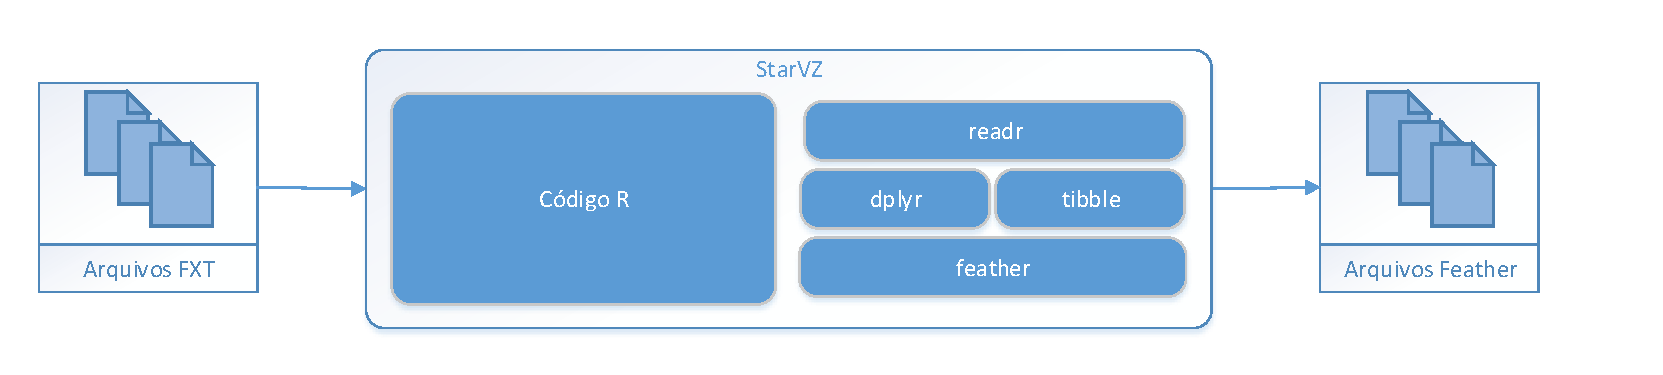
\includegraphics[width=1\textwidth]{./img/starvz-arch.pdf}}
 \caption{Arquitetura da aplicação StarVZ.}
 \label{fig:starvz-app}
\end{figure}

Durante o trabalho, identificou-se que não havia uma biblioteca que suportasse a escrita de tabelas Spark em arquivos \texttt{Feather}.
Isso é essencial para compararmos a escrita do mesmo tipo de dados tanto na execução sequencial quanto na distribuída utilizando tabelas Spark.
Devido ao ecossistema Hadoop utilizar o formato \texttt{Parquet} \cite{} como padrão para armazenamento de dados colunares, a aplicação 
foi adaptada para escrever suas saídas neste formato. Isso foi realizado utilizando a biblioteca Apache arrow \cite{}, a arquitetura final da aplicação sequencial pode ser visualizada na Figura \ref{fig:starvz-app-arrow}. 

\begin{figure}[ht]
 \centerline{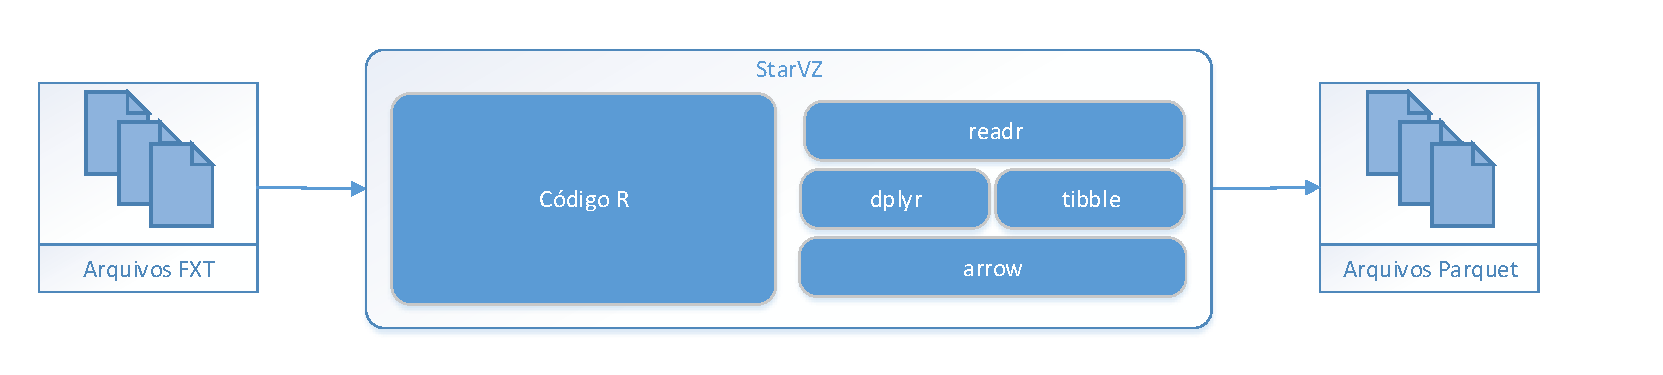
\includegraphics[width=1\textwidth]{./img/starvz-arch-arrow.pdf}}
 \caption{Arquitetura da aplicação StarVZ adaptada para escrever Parquet.}
 \label{fig:starvz-app-arrow}
\end{figure}

Considerando o tamanho dos arquivos de entrada, utilizaremos o HDFS para armazená-los. Dessa forma, a leitura dos arquivos 
também utilizaremos a capacidade de leitura distribuída das entradas. O \texttt{Gerenciador de Cluster} inicialmente trabalharemos


\section{Implementação} \label{sect:implement}
